\subsubsection{Simulation des angepassten Netzwerks}
\label{chap:Simulation des angepassten Netzwerks}

Im Folgenden werden einige Simulationen des in Simulink implementierten \ac{hnn} beschrieben, eine Validierung der Funktionsweise des Netzwerkes ist im Anhang \ref{app:Umsetzung des Hopfield-Netzwerks in Simulink} zu finden. Die Gewichte werden einmalig zufällig generiert und mit diesen Werten in allen weiteren Simulationen weitergearbeitet. Es sollen also keine sinnvollen Anwendungen getestet, sondern ausschließlich die Formen der Ausgaben überprüft werden.

Die erste Simulation wird mit \(\beta=0\) und \(\vec{d}=(1,1,1)\) durchgeführt. Der Vektor \(\vec{d}\) steht dabei für die Eingabe in das Netzwerk bzw. die erwartete Ausgabe. Die Gewichte werden mit \((-1.21,1.319,0.3204)\) zufällig erzeugt. Wie in Abbildung \ref{fig:Simulation HNN 1} zu sehen, gibt das Netzwerk zu Beginn der Simulation für alle Zustände einen Wert zwischen \(0.7\) und \(0.75\) aus, da für alle Zustände der Initialwert \(1\) gesetzt wurde und \(\rho(1)\approx{0.7311}\) gilt. Das Netzwerk findet einen Fixpunkt bei \(y\approx{(0.51,0.47,0.55)}\), bei dem auch die Energiefunktion ihren niedrigsten Wert erreicht. Die Kostenfunktion steigt proportional zur Energiefunktion, da sich die Ausgabe des Modells immer weiter von der Eingabe \(\vec{d}=(1,1,1)\) entfernt.

\begin{figure}[h]
  \caption{Erste Simulation des \ac{hnn}}
  \centering
  \begin{subfigure}[b]{0.32\textwidth}
    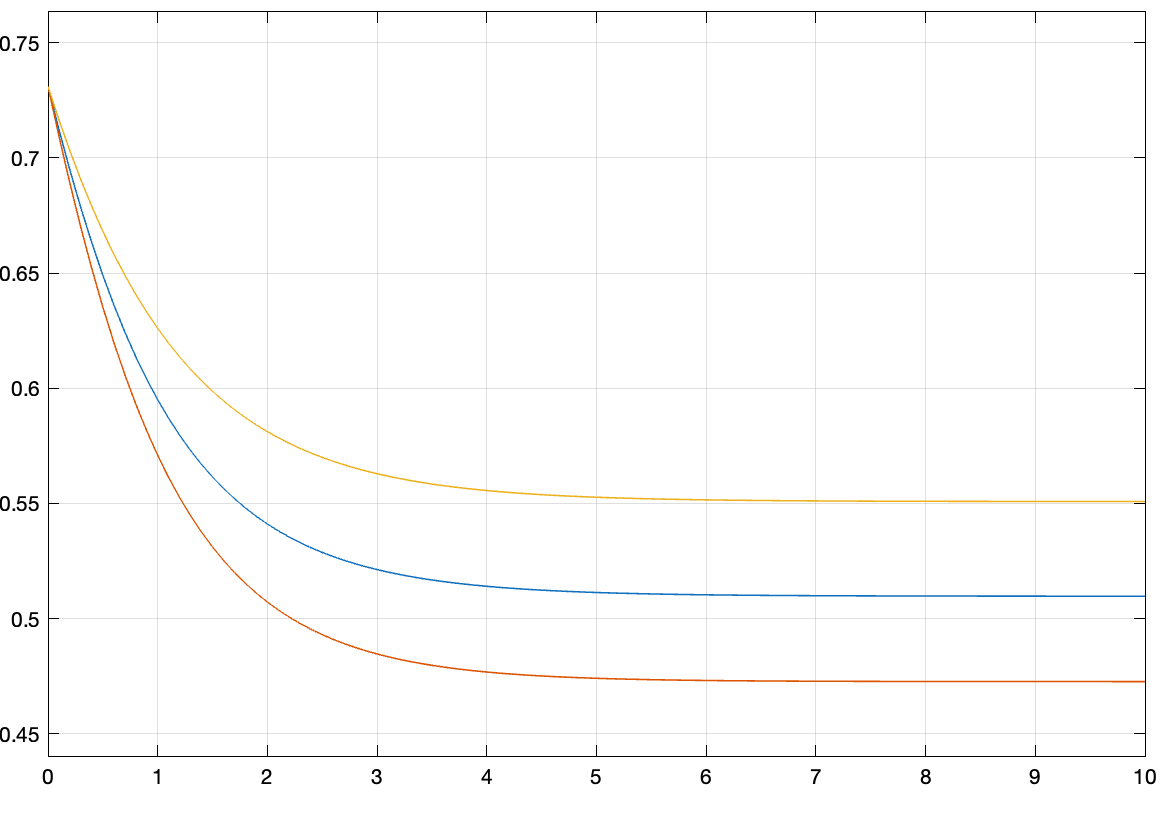
\includegraphics[width=\textwidth]{abbildungen/hnn_simulation_1_ausgabe.png}
    \caption{Ausgabe}
  \end{subfigure}%
  \hfill
  \begin{subfigure}[b]{0.32\textwidth}
    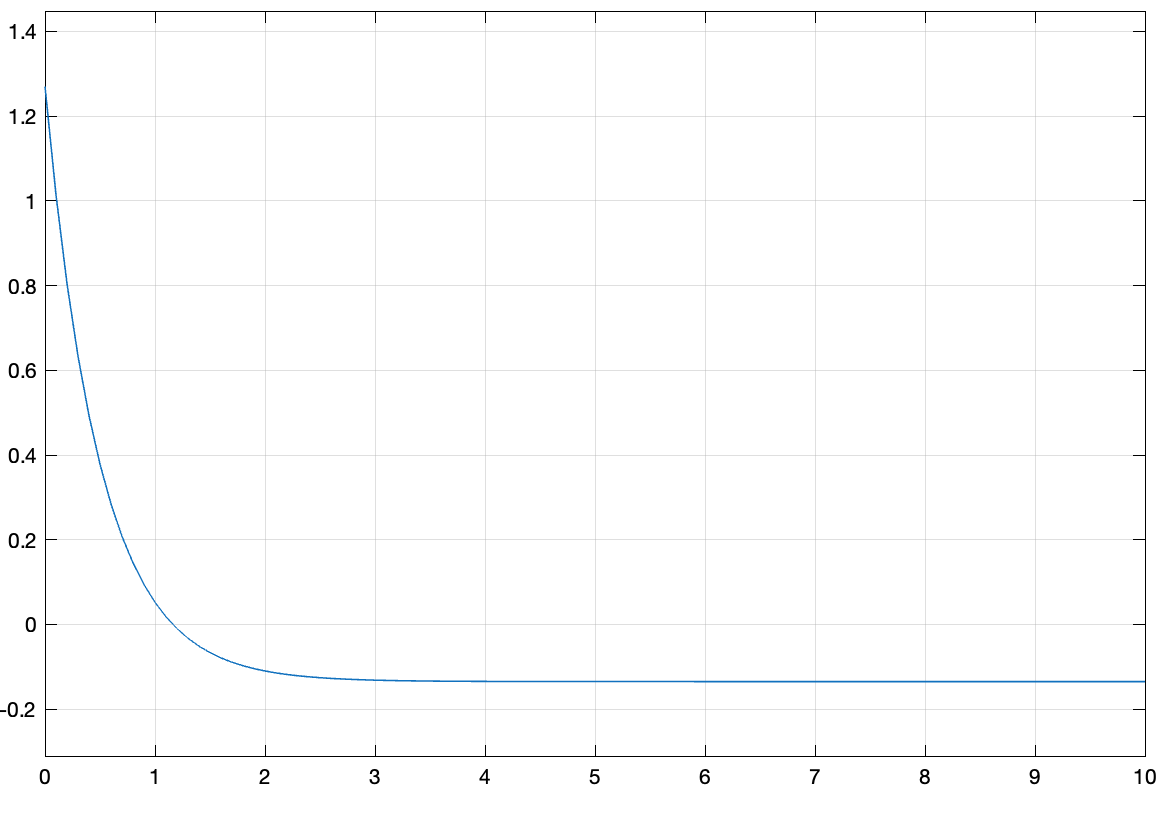
\includegraphics[width=\textwidth]{abbildungen/hnn_simulation_1_energiefunktion.png}
    \caption{Energie}
  \end{subfigure}%
  \hfill
  \begin{subfigure}[b]{0.32\textwidth}
    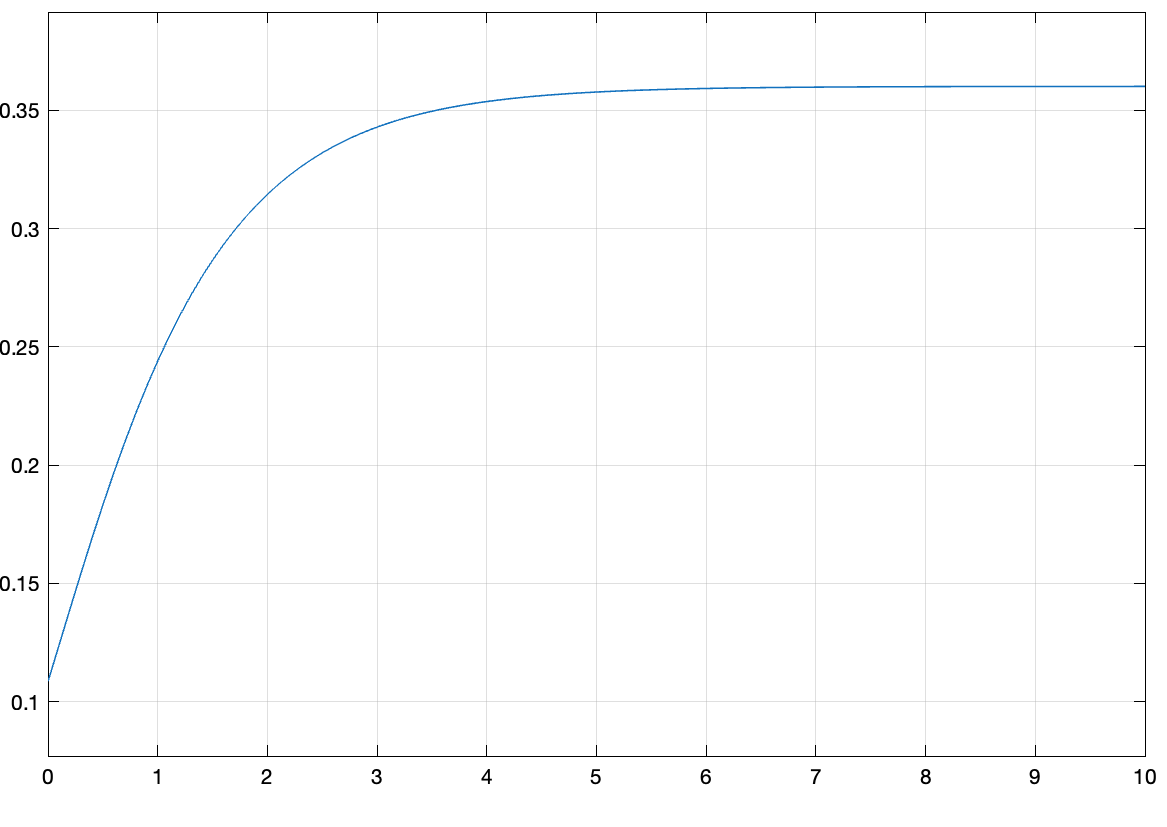
\includegraphics[width=\textwidth]{abbildungen/hnn_simulation_1_kostenfunktion.png}
    \caption{Kosten}
  \end{subfigure}
  \\
  Quelle: Eigene Darstellung
  \label{fig:Simulation HNN 1}
\end{figure}

Für die zweite Simulation wird die Eingabe zu \(\vec{d}=(1,0,0)\) geändert. Da das \ac{hnn} die Eigenschaften eines assoziativen Speichers besitzt (vgl. Kapitel \ref{chap:Das Hopfield-Netzwerk: Eine Herangehensweise an neuronale Netze}), ist zu erwarten, dass das Netzwerk die gleiche Ausgabe wie aus der vorherigen Simulation liefert. Diese These lässt sich, wie in Abbildung \ref{fig:Simulation HNN 2} gezeigt, bestätigen.

\begin{figure}[h]
  \caption{Zweite Simulation des \ac{hnn}}
  \centering
  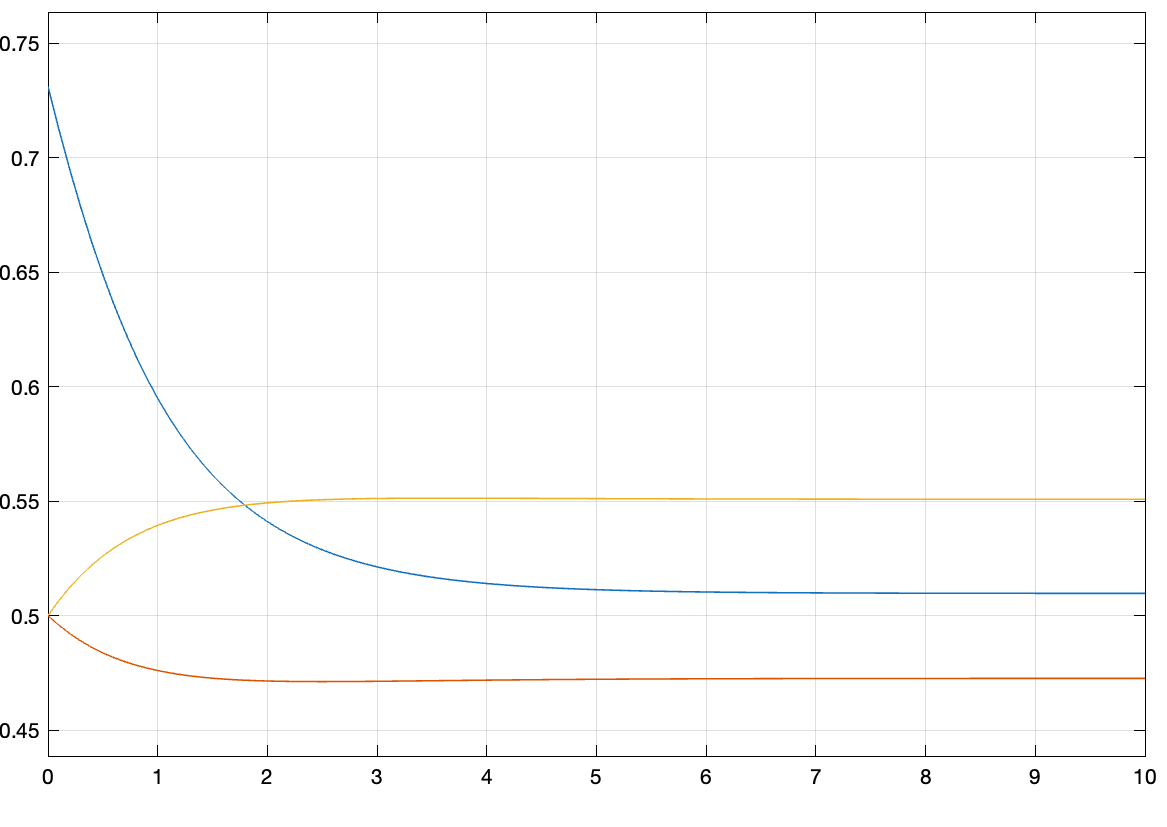
\includegraphics[width=0.5\textwidth]{abbildungen/hnn_simulation_2_ausgabe.png}
  \\
  Quelle: Eigene Darstellung
  \label{fig:Simulation HNN 2}
\end{figure}

Die dritte Simulation wird mit \(\beta=1\) durchgeführt, wodurch die Zustände des Netzwerks höhere Werte annehmen und somit die Kostenfunktion kleiner sein sollte. Dementsprechend sollte die Energiefunktion auch einen höheren Wert annehmen, da die Ausgabe des Netzwerks vom optimalen Ergebnis aus der ersten Simulation abweicht. Die Ergebnisse der Simulation (siehe Abbildung \ref{fig:Simulation HNN 3}) bestätigen diese Annahmen.

\begin{figure}[h]
  \caption{Dritte Simulation des \ac{hnn}}
  \centering
  \begin{subfigure}[b]{0.32\textwidth}
    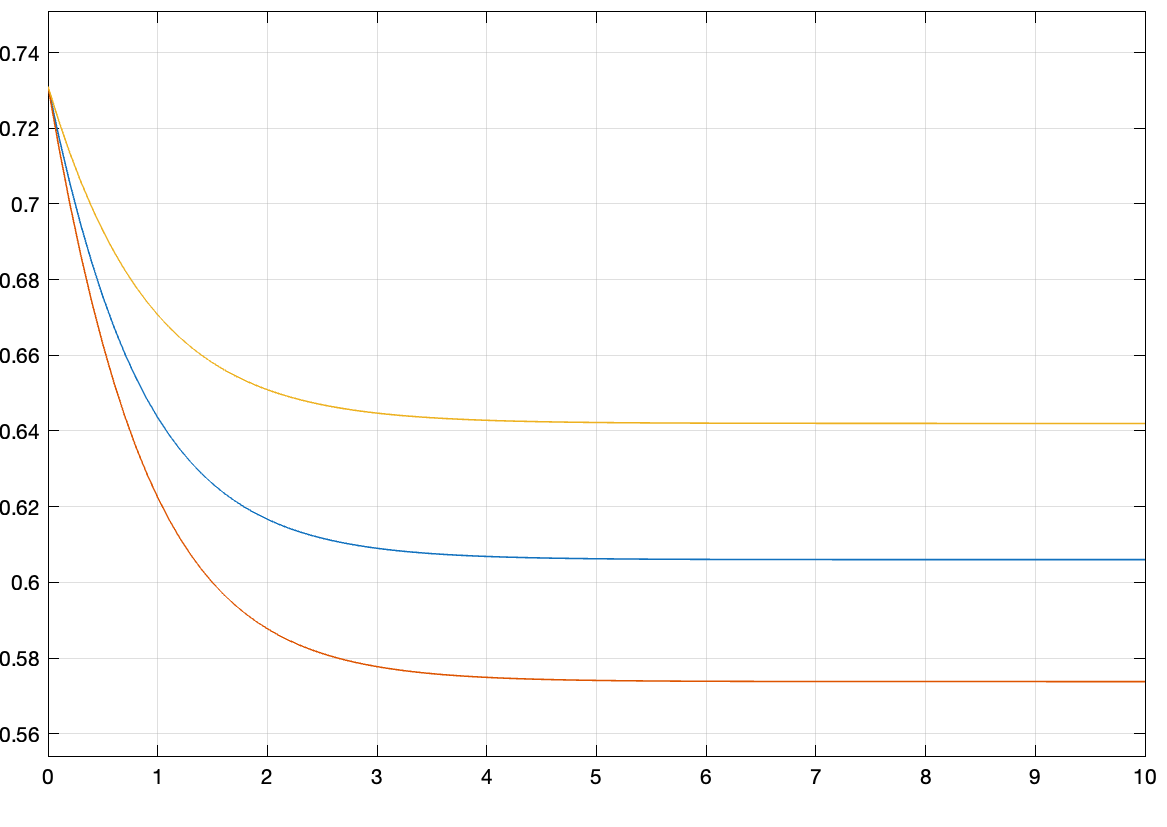
\includegraphics[width=\textwidth]{abbildungen/hnn_simulation_3_ausgabe.png}
    \caption{Ausgabe}
  \end{subfigure}%
  \hfill
  \begin{subfigure}[b]{0.32\textwidth}
    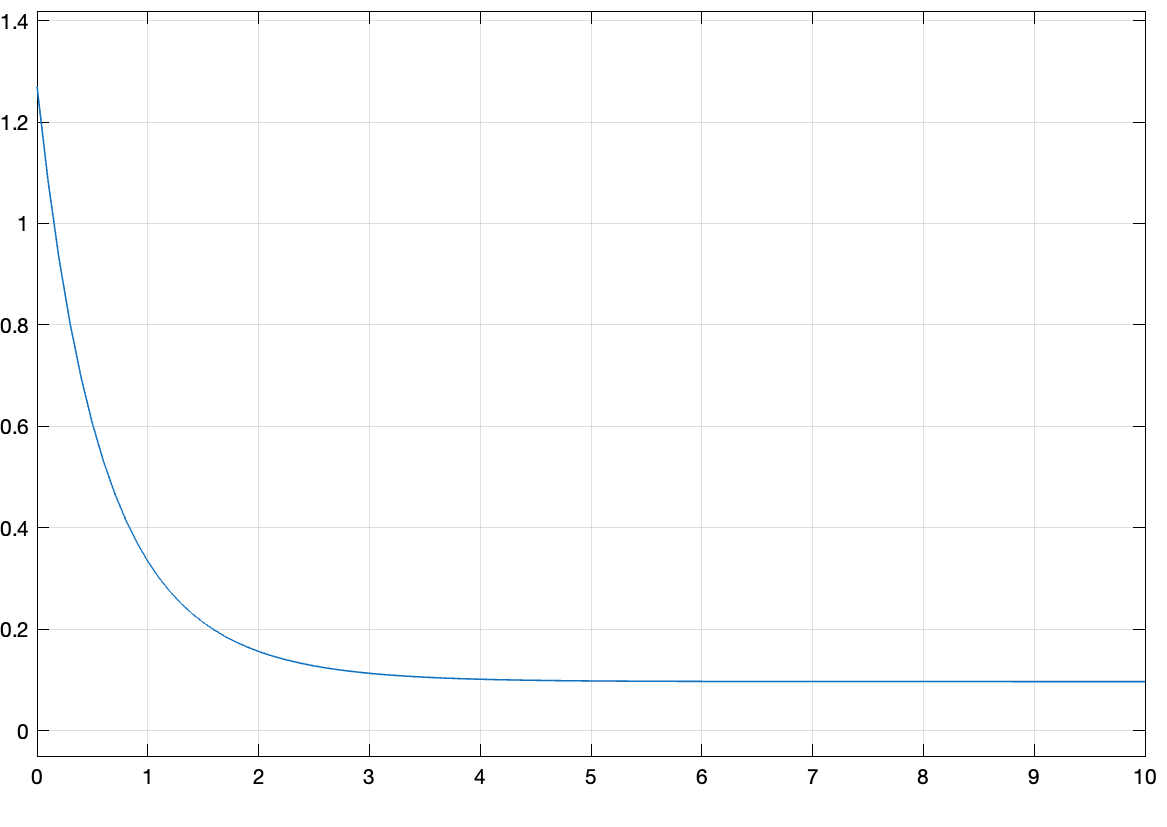
\includegraphics[width=\textwidth]{abbildungen/hnn_simulation_3_energiefunktion.png}
    \caption{Energie}
  \end{subfigure}%
  \hfill
  \begin{subfigure}[b]{0.32\textwidth}
    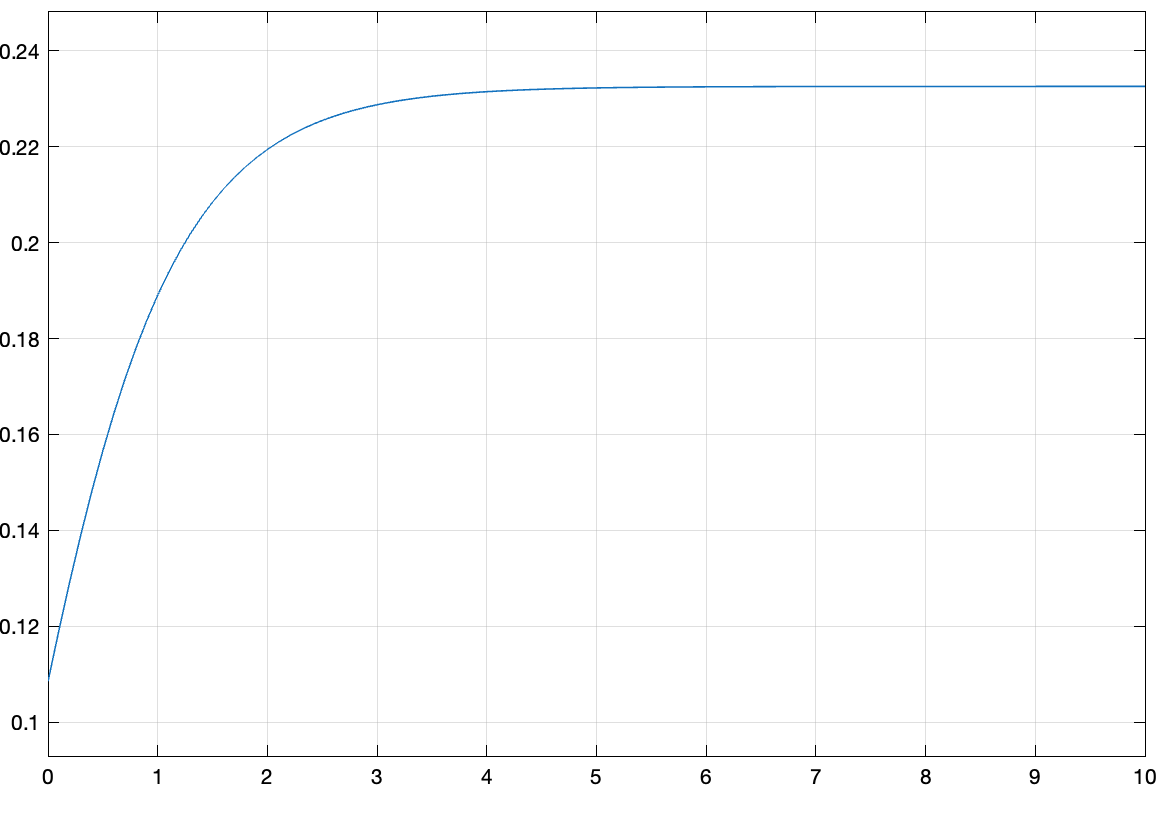
\includegraphics[width=\textwidth]{abbildungen/hnn_simulation_3_kostenfunktion.png}
    \caption{Kosten}
  \end{subfigure}
  \\
  Quelle: Eigene Darstellung
  \label{fig:Simulation HNN 3}
\end{figure}
